%!TEX root = ../report.tex
\chapter{Experiments and Results}
\label{cha:Experiments}

\section{Experimental Plan}
\label{sec:experimentalPlan}
The goal of the experiments is to gather data for comparison of search methods. when comparing search methods, speed and accuracy will be the metrics used. Three methods for searching is used, one following all gathering all objects connected to an input subject, regardless of the predicate. One method following Yago predicates leading directly to a Yago URI. And the final method will follow the same predicates as the second, and will also add a condition where all nodes must match at least one query word.

\subsection{Time}
When timing the search, two different times will be measured, time for each query, and time for each root node. In addition to these, avg. nodes visited for each root will also be used. Taking the average of these over a large input set should generate an appropriate result. Both time metrics measure how fast results are found, so the results should be similar as long as the input data does not contain a high number of highly connected nodes.

The timing of the algorithm should be the same as any breath first search, $\Theta(\mathsf{V} + \mathsf{E})$ so that the best case is visiting only the first vertex, and the worst case is traversing the entire graph.


\subsection{Scoring and ranking}
Each query is given a score. This score will be used to see how pruning, and difference in predicates can lead to differences in the result tree. Two metrics for accuracy will be used, avg. accuracy for each result and avg. highest accuracy for each query.

\subsubsection{BFS}

\subsubsection{BFS with pruning}

% -------------------------------------------------------------------- %
\section{Experimental Setup}
\label{sec:experimentalSetup}

\section{Data set}
When selecting a data set an important feature was accurate spatial and temporal data. For this Yago was selected. Yago allows for download of subsets of data, and contains all the necessary data. The high accuracy in Yago was also a benefit of this data set. From Yago, the data selected was the entire Yago taxonomy, the entire Yago core, and from Genomes the sets GeonamesOnlyData, GeonamesClassIds, GeonamesGlosses, GeonamesTypes, and GeonamesClasses were selected. These sets makes it possible to build a complete graph of the entities in Yago, but keeps the disk usage as low as possible.\\

- Short description of each of the parts\\
- preprocessing: replace non-unicode chars, replacing space with underscore in URIs, terminate triplet where missing termination, remove double quotes in URIs, remove backslash unless legal escape sequence\\
- tdbloader for persistent queryable storage\\
- Structure of graph? Here or in Yago description?\\
% awk -F ' ' '{a[$1] += $2} END{for (i in a) print i, a[i]}' topMiddle100stemmed.txt | sort -k 2 -n > topMiddle.txt


\section{Queries}
When selecting the keywords used in queries, a semi random selection method was used at first. This method created three pools of words, rare words (less than 1000 occurrences) uncommon words (less than 100 000 occurrences) and common words (more than 100 000 occurrences). The three pools where created by stemming all words, then counting occurrences. From each pool of words, a set of 100 where randomly selected, and from those 100, 10 where selected manually to ensure a range of occurrences, and to ensure no stop words, misspelled words or other errors were in the final set of keywords.\\

A second set of words were also chosen to ensure a larger hit rate. This set was a random selection of 20 words from the top 150 words. From the 20 random words 10 where manually selected, the 150 word number was selected based on Zipfs law \cite{zipf}.\\

When selecting places for spatial queries, a set of 20 random places were selected from the YagoGeonamesOnlyData set, and from that set, 5 were chosen manually for the final set. In the final set, three places where added manually, Oslo, London, and New York City were added to ensure variation in placement and node connections.\\

Generating random queries can create results that will not have any hits.\\
Find a good method of creating queries.\\

\section{Pruning}
A simple method to improve performance when searching in large data sets is to remove data that is unnecessary to search.

\subsection{Predicate pruning}
Predicate pruning is the process of eliminating predicates from the search. The taxonomy of Yago creates assigns predicates to one or more group or class. By selecting specific groups or classes it is possible to follow the types of data searched for, while eliminating a lot of other data. When pruning based on classes or groups the type of data returned must be known beforehand, to ensure that no possible hits is overlooked.\\

Another possible method for pruning is to specify the exact predicates to follow. This will remove a lot of data, but is possibility when searching for something specific. This will also greatly increase the speed of the search, and reduce the memory usage for the search. 


% -------------------------------------------------------------------- %
\section{Experimental Results}
\label{sec:experimentalResults}

\section{BFS search}
BFS search without any pruning and search depth of 3 were unable to finish due to memory constraints and taking too long. Search with a depth of 2 may finish, depending on on the connectedness of the nodes discovered, and the amount of root nodes found in the search.

\subsection{Time}
When running the query, two sets are displayed, one with mostly random input data, and one with more closely selected data.

Because most of the randomly selected places had few possible root nodes, the table contains only the manually selected.

- time/query \\
- time/root \\
- roots found/ query \\

- accuracy/ result\\
- avg highest accuracy/ query\\

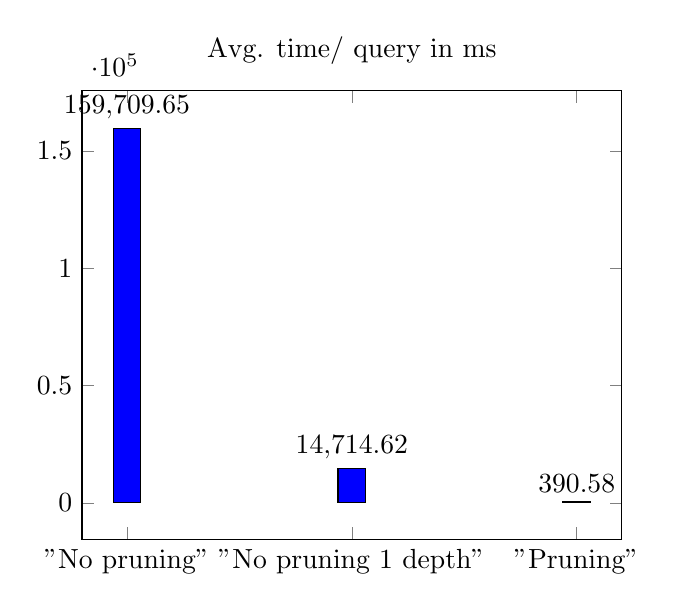
\begin{tikzpicture}
\begin{axis}[
	title={Avg. time/ query in ms},
	every axis plot post/.style={/pgf/number format/fixed},
	symbolic x coords={"No pruning", "No pruning 1 depth", "Pruning"},
	visualization depends on=rawy\as\rawy, % Save the unclipped values
	nodes near coords={\pgfmathprintnumber{\rawy}},
    xtick=data]
    \addplot[ybar,fill=blue] coordinates {("No pruning",159709.6486) ("No pruning 1 depth",14714.6216) ("Pruning",390.5810)};
\end{axis}
\end{tikzpicture}
%
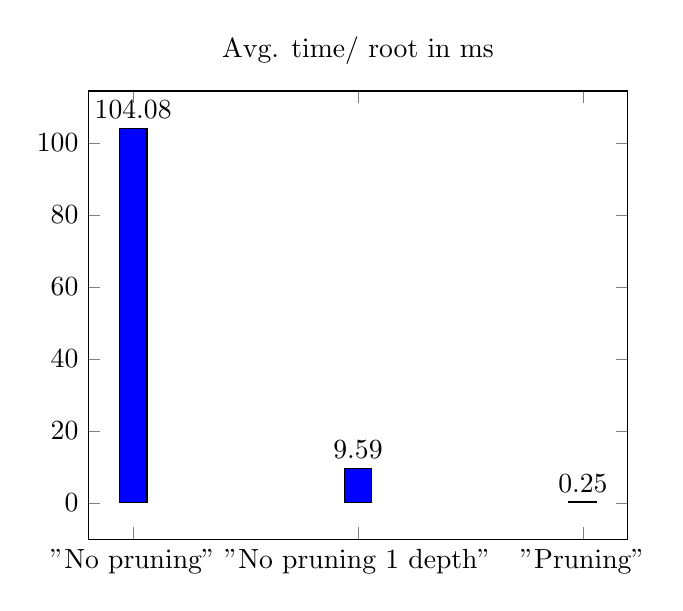
\begin{tikzpicture}
\begin{axis}[
	title={Avg. time/ root in ms},
	every axis plot post/.style={/pgf/number format/fixed},
	symbolic x coords={"No pruning", "No pruning 1 depth", "Pruning"},
	visualization depends on=rawy\as\rawy, % Save the unclipped values
	nodes near coords={\pgfmathprintnumber{\rawy}},
    xtick=data]
    \addplot[ybar,fill=blue] coordinates {("No pruning",104.08202) ("No pruning 1 depth",9.58944) ("Pruning",0.2545398)};
\end{axis}
\end{tikzpicture}


\subsection{Accuracy}

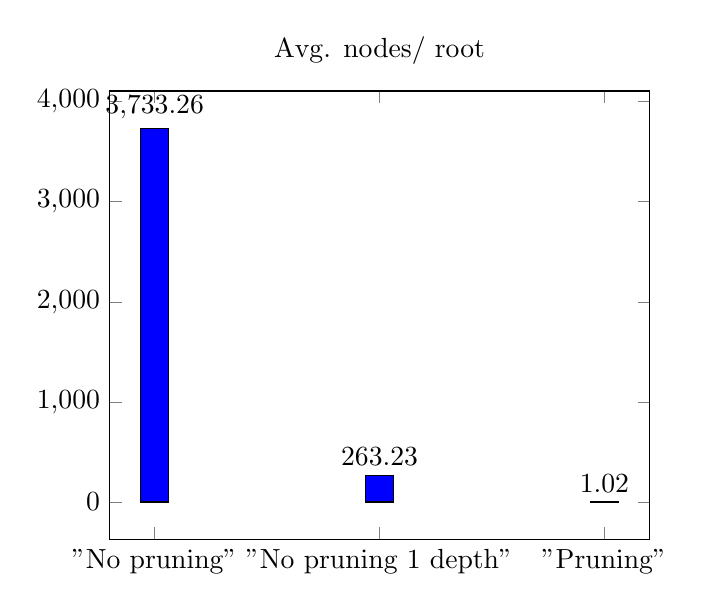
\begin{tikzpicture}
\begin{axis}[
	title={Avg. nodes/ root},
	every axis plot post/.style={/pgf/number format/fixed},
	symbolic x coords={"No pruning", "No pruning 1 depth", "Pruning"},
	visualization depends on=rawy\as\rawy, % Save the unclipped values
	nodes near coords={\pgfmathprintnumber{\rawy}},
    xtick=data]
    \addplot[ybar,fill=blue] coordinates {("No pruning",3733.2554) ("No pruning 1 depth",263.2276) ("Pruning",1.0220)};
\end{axis}
\end{tikzpicture}
%
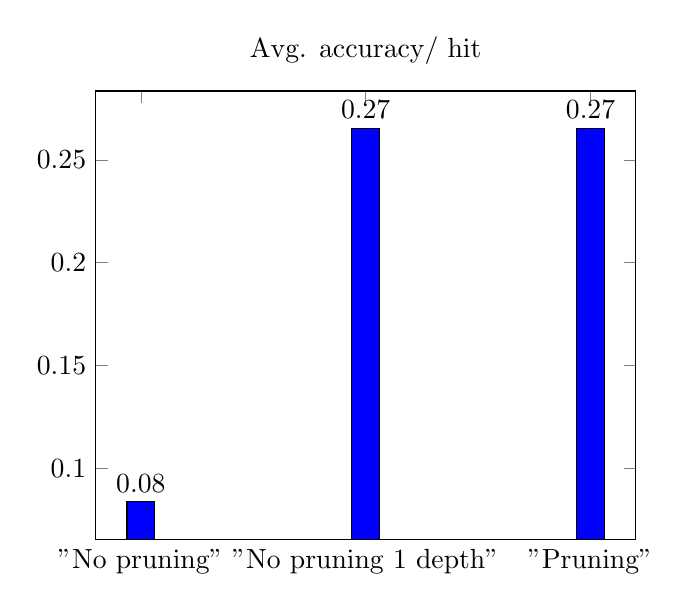
\begin{tikzpicture}
\begin{axis}[
	title={Avg. accuracy/ hit},
	every axis plot post/.style={/pgf/number format/fixed},
	symbolic x coords={"No pruning", "No pruning 1 depth", "Pruning"},
	visualization depends on=rawy\as\rawy, % Save the unclipped values
	nodes near coords={\pgfmathprintnumber{\rawy}},
    xtick=data]
    \addplot[ybar,fill=blue] coordinates {("No pruning",0.08353006) ("No pruning 1 depth",0.2654491) ("Pruning",0.26523)};
\end{axis}
\end{tikzpicture}
%
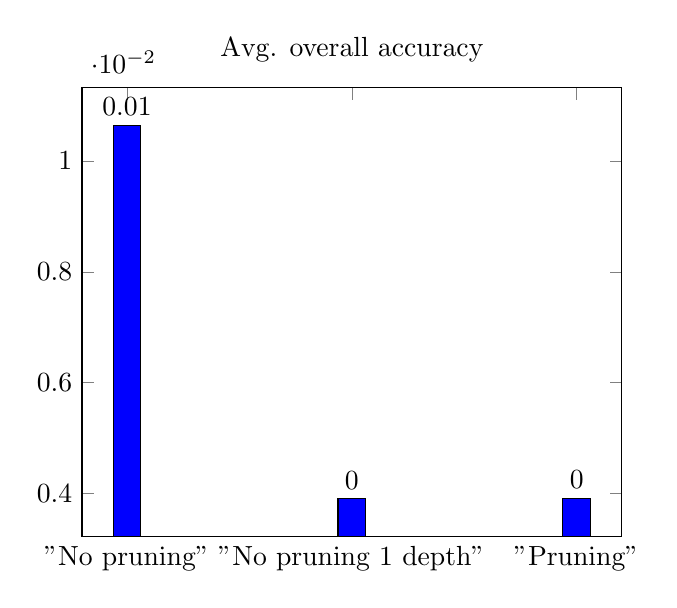
\begin{tikzpicture}
\begin{axis}[
	title={Avg. overall accuracy},
	every axis plot post/.style={/pgf/number format/fixed},
	symbolic x coords={"No pruning", "No pruning 1 depth", "Pruning"},
	visualization depends on=rawy\as\rawy, % Save the unclipped values
	nodes near coords={\pgfmathprintnumber{\rawy}},
    xtick=data]
    \addplot[ybar,fill=blue] coordinates {("No pruning",0.01064373) ("No pruning 1 depth",0.0039040070) ("Pruning",0.00390785)};
\end{axis}
\end{tikzpicture}
%
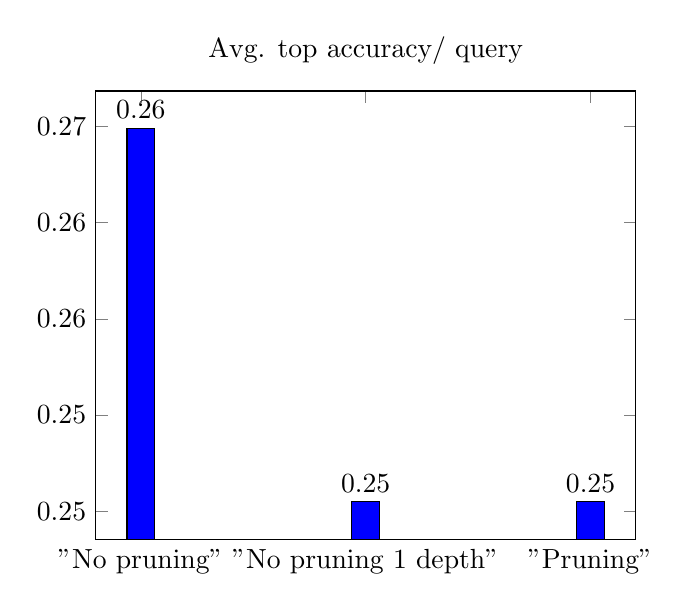
\begin{tikzpicture}
\begin{axis}[
	title={Avg. top accuracy/ query},
	every axis plot post/.style={/pgf/number format/fixed},
	symbolic x coords={"No pruning", "No pruning 1 depth", "Pruning"},
	visualization depends on=rawy\as\rawy, % Save the unclipped values
	nodes near coords={\pgfmathprintnumber{\rawy}},
    xtick=data]
    \addplot[ybar,fill=blue] coordinates {("No pruning",0.2648955) ("No pruning 1 depth",0.245495) ("Pruning",0.24549)};
\end{axis}
\end{tikzpicture}

\glsresetall
